\documentclass[12pt]{article}
\usepackage[utf8]{inputenc}
\usepackage[dvips]{graphicx}
\usepackage{epsfig}
\usepackage{fancybox}
\usepackage{verbatim}
\usepackage{array}
\usepackage{latexsym}
\usepackage{alltt}
\usepackage{amssymb}
\usepackage{amsmath}
\usepackage{hyperref}
\usepackage{listings}
\usepackage{color}
\usepackage{algorithm}
\usepackage{algpseudocode}
\usepackage[hmargin=3cm,vmargin=5.0cm]{geometry}
\usepackage{epstopdf}
\usepackage{caption}
\usepackage{tikz}
\usepackage{pgfplots}
\usepackage{amsmath}
\pgfplotsset{width=8cm,compat=1.9}
\usepackage{multirow}
\usepackage{graphicx}
\graphicspath{ {./images/} }
\topmargin=-1.8cm
\addtolength{\textheight}{6.5cm}
\addtolength{\textwidth}{2.0cm}
\setlength{\oddsidemargin}{0.0cm}
\setlength{\evensidemargin}{0.0cm}
\newcommand{\HRule}{\rule{\linewidth}{1mm}}
\newcommand{\kutu}[2]{\framebox[#1mm]{\rule[-2mm]{0mm}{#2mm}}}
\newcommand{\gap}{ \\[1mm] }
\newcommand{\Q}{\raisebox{1.7pt}{$\scriptstyle\bigcirc$}}
\newcommand{\minus}{\scalebox{0.35}[1.0]{$-$}}

\lstset{
    %backgroundcolor=\color{lbcolor},
    tabsize=2,
    language=MATLAB,
    basicstyle=\footnotesize,
    numberstyle=\footnotesize,
    aboveskip={0.0\baselineskip},
    belowskip={0.0\baselineskip},
    columns=fixed,
    showstringspaces=false,
    breaklines=true,
    prebreak=\raisebox{0ex}[0ex][0ex]{\ensuremath{\hookleftarrow}},
    %frame=single,
    showtabs=false,
    showspaces=false,
    showstringspaces=false,
    identifierstyle=\ttfamily,
    keywordstyle=\color[rgb]{0,0,1},
    commentstyle=\color[rgb]{0.133,0.545,0.133},
    stringstyle=\color[rgb]{0.627,0.126,0.941},
}


\begin{document}

\noindent
\HRule %\\[3mm]
\small
\begin{center}
	\LARGE \textbf{CENG 483} \\[4mm]
	\Large Introduction to Computer Vision \\[4mm]
	\normalsize Spring 2018-2019 \\
	\Large Take Home Exam 1 \\
	\Large Content Based Image Retrieval \\
    \Large Student Random ID: 70 \\
\end{center}
\HRule

\begin{center}
\end{center}
\vspace{-10mm}
\noindent\\ \\ 
Please fill in the sections below only with the requested information. If you have additional things you want the mention, you can use the last section. Please note that all of the results in this report should be given for the \textbf{validation set}.
\section{Grayscale Histogram}
In this section, give your results only for grid level 1.

\begin{itemize}
\item Pick 5 different quantization levels and give your mAP results for each of them.
\item What do you think caused the difference between mAP for these?
\end{itemize}

I evaluated the given queries with the dataset by using grayscale histogram with 8 different quantization levels (i.e. bin counts) for grid level 1. Mean Average Precisions (mAP) of each quantization level are below:

\begin{minipage}{\textwidth}
	\begin{minipage}{0.49\textwidth}
		\centering
		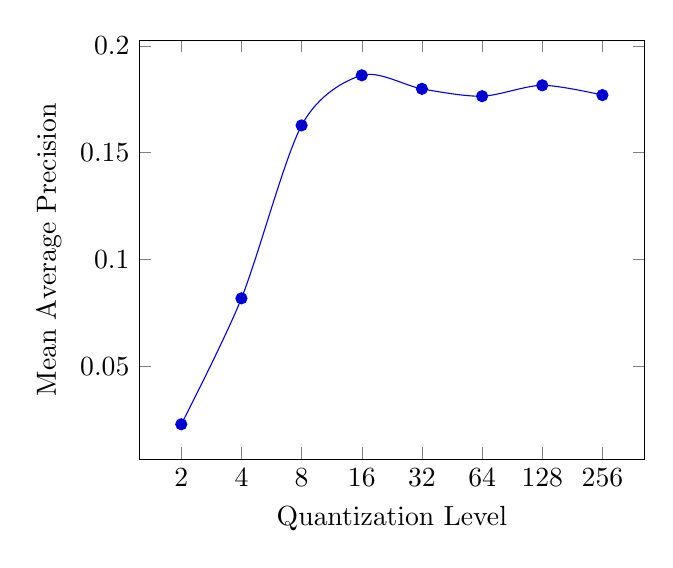
\begin{tikzpicture}
		    \begin{axis}
		        [
		        ,xlabel=Quantization Level
		        ,ylabel=Mean Average Precision
		        ,yticklabel style={/pgf/number format/fixed}
		        ,xtick=data,
		        ,xticklabels={2, 4,8, 16, 32, 64, 128, 256}
		        ]
		        \addplot+[smooth] coordinates
		        {(0,0.02276) (1,0.08175) (2,0.16273) (3,0.18619) (4,0.17984) (5,0.17641) (6,0.18151) (7,0.17693)};
		    \end{axis}
		\end{tikzpicture}
		\captionsetup{width=.9\textwidth}
		\captionof{figure}{Mean Average Precision with different quantization levels for grid level 1 grayscale histogram}
	 \end{minipage}
	 \hfill
	\begin{minipage}{0.49\textwidth}
		\centering
		\begin{tabular}{ | c | c | }
		  \hline			
		  \bf Bin & \bf mAP \\
		  \hline		
		  2 & 0.02276 \\
		  \hline	
		  4 & 0.08175 \\
		  \hline	
		  8 & 0.16273 \\
		  \hline	
		  16 & 0.18619 \\
		  \hline	
		  32 & 0.17984 \\
		  \hline	
		  64 & 0.17641 \\
		  \hline	
		  128 & 0.18151 \\
		  \hline	
		  256 & 0.17693 \\
		  \hline
		\end{tabular}
		\captionsetup{width=.8\textwidth}
		\captionof{table}{Mean Average Precision with different quantization levels for grid level 1 grayscale histogram}
	\end{minipage}
\end{minipage}

It is obvious that lower quantization levels such as 1, 2, 4 have lower mAP as each bin corresponds to large interval of grayscaled value, and this doens't result in distinguishing the differences in different images. I've expected same result with large number of bin count such as 256; however, 256 bin count has slight difference with the best configuration in this part. 256 bin count's mAP is 0.17693 whereas the best configuration which is 16 bin count's mAP is 0.18619.

\section{3D RGB Histogram}
In this section, give your results only for grid level 1.

\begin{itemize}
\item Pick 5 different quantization levels and give your mAP results for each of them.
\item What do you think caused the difference between mAP for these?
\end{itemize}

\begin{minipage}{\textwidth}
	\begin{minipage}{0.49\textwidth}
		\centering
		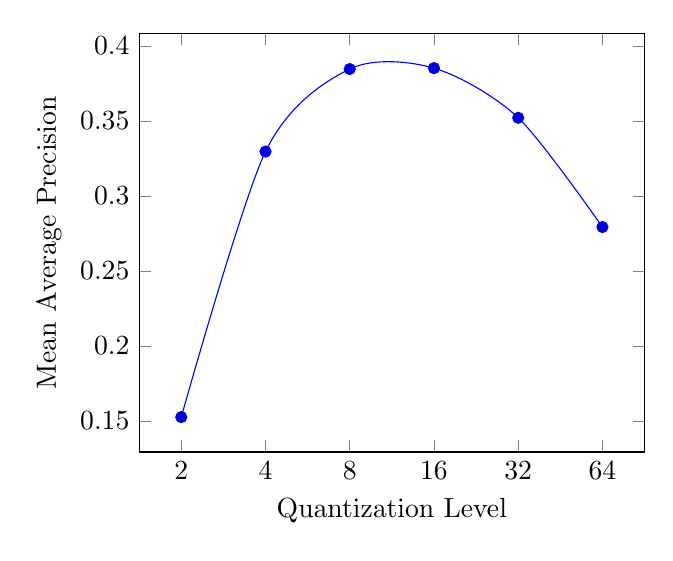
\begin{tikzpicture}
		    \begin{axis}
		        [
		        ,xlabel=Quantization Level
		        ,ylabel=Mean Average Precision
		        ,yticklabel style={/pgf/number format/fixed}
		        ,xtick=data,
		        ,xticklabels={2, 4, 8, 16, 32, 64}
		        ]
		        \addplot+[smooth] coordinates
		        {(0,0.15246) (1,0.32950) (2,0.38451) (3,0.38512) (4,0.35201) (5,0.27919)};
		    \end{axis}
		\end{tikzpicture}
		\captionsetup{width=.9\textwidth}
		\captionof{figure}{Mean Average Precision with different quantization levels for grid level 1 gradient histogram}
	 \end{minipage}
	 \hfill
	\begin{minipage}{0.49\textwidth}
		\centering
		\begin{tabular}{ | c | c | }
		  \hline			
		  \bf Bin & \bf mAP \\
		  \hline		
		  2 & 0.15246 \\
		  \hline	
		  4 & 0.32950 \\
		  \hline	
		  8 & 0.38451 \\
		  \hline	
		  16 & 0.38512 \\
		  \hline	
		  32 & 0.35201 \\
		  \hline	
		  64 & 0.27919 \\
		  \hline
		\end{tabular}
		\captionsetup{width=.8\textwidth}
		\captionof{table}{Mean Average Precision with different quantization levels for grid level 1 gradient histogram}
	\end{minipage}
\end{minipage}

\section{Gradient Histogram}

\begin{itemize}
\item Which method did you use for obtaining the gradients? Explain the steps of the method briefly.
\item Visualize some of your intermediate results (filtered versions of the image).
\item Pick 3 different quantization levels for your histogram and give your mAP results for each of them.
\item What do you think caused the difference between mAP for these?
\end{itemize}



\begin{minipage}{\textwidth}
	\begin{minipage}{0.49\textwidth}
	\[\text{Horizontal-Filter-0: }
	\begin{bmatrix}
	    -1 & 0 & 1 \\
	    -1 & 0 & 1 \\
	    -1 & 0 & 1
	\end{bmatrix}
	\]
	\linebreak
	\[
	\text{Vertical-Filter-0: }
	\begin{bmatrix}
	    1 & 1 & 1 \\
	    0 & 0 & 0 \\
	    -1 & -1 & -1
	\end{bmatrix}
	\]
	\end{minipage}
	\begin{minipage}{0.25\textwidth}
	\[\text{Horizontal-Filter-1: }
	\begin{bmatrix}
	    -1 & 0 & 1 \\
	    -2 & 0 & 2 \\
	    -1 & 0 & 1
	\end{bmatrix}
	\]
	\linebreak
	\[
	\text{Vertical-Filter-1: }
	\begin{bmatrix}
	    1 & 2 & 1 \\
	    0 & 0 & 0 \\
	    -1 & -2 & -1
	\end{bmatrix}
	\]
	\end{minipage}
\end{minipage}

\begin{figure}[h]
	\centering
	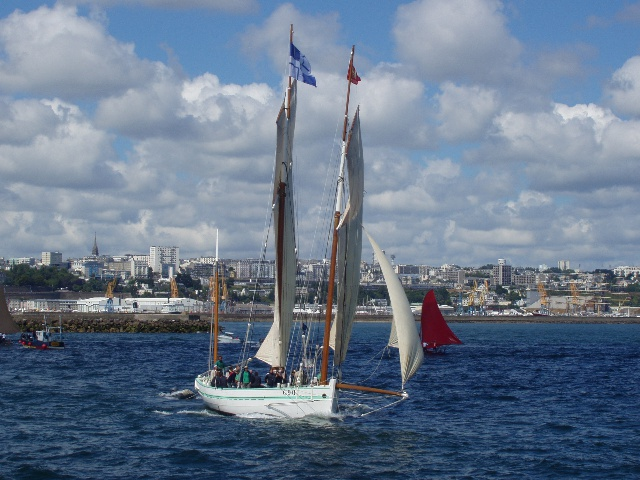
\includegraphics[width=0.49\textwidth]{IAcBBqAmEI.jpg}
	\caption{Example image from the dataset}
\end{figure}

\begin{minipage}{\textwidth}
	\begin{minipage}{0.49\textwidth}
		\centering
		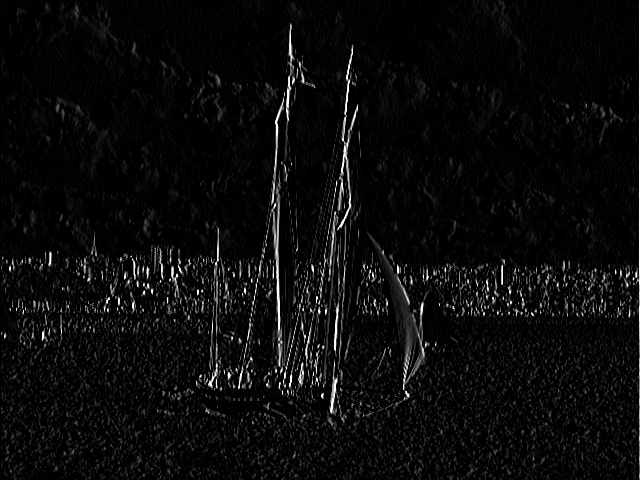
\includegraphics[width=0.8\textwidth]{IAcBBqAmEI_horizontal-0.jpeg}
		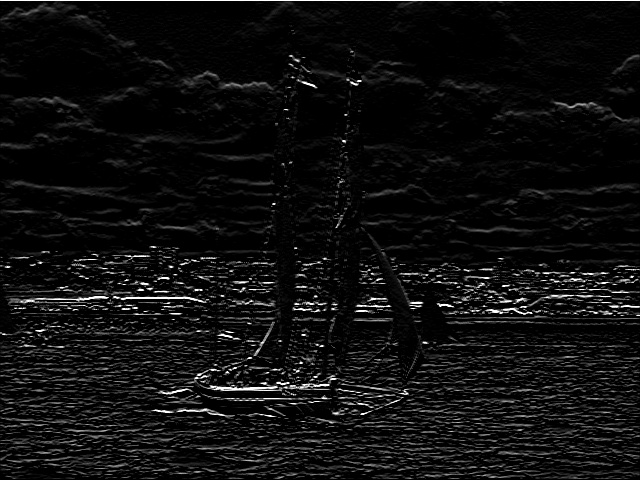
\includegraphics[width=0.8\textwidth]{IAcBBqAmEI_vertical-0.jpeg}
		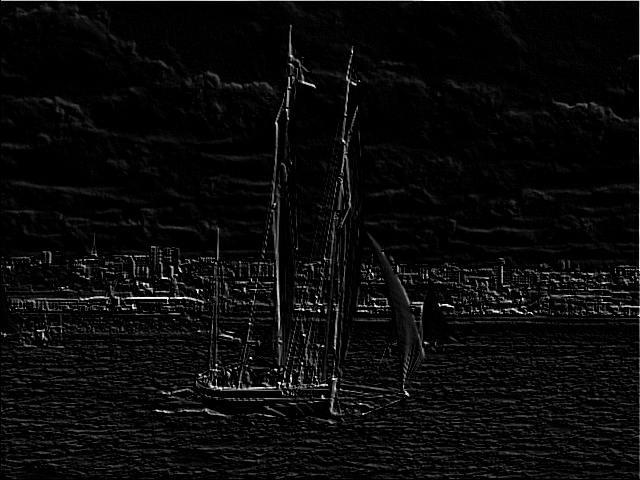
\includegraphics[width=0.8\textwidth]{IAcBBqAmEI_blended-0.jpeg}
		\captionsetup{width=.8\textwidth}
		\captionof{figure}{Horizontally, vertically filtered images and their blend, Filter-0}
	\end{minipage}
	\begin{minipage}{0.49\textwidth}
		\centering
		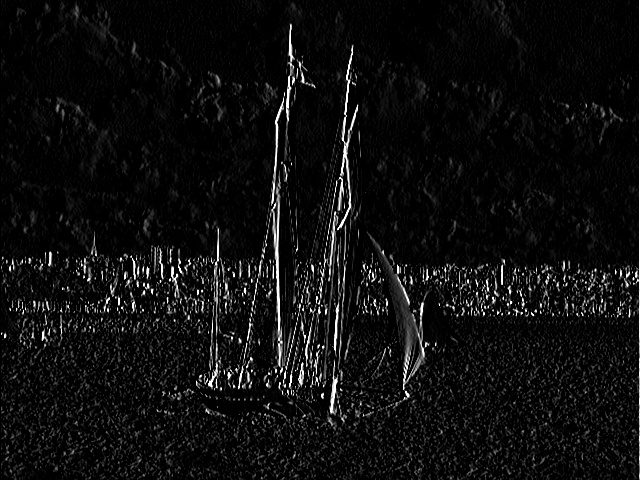
\includegraphics[width=0.8\textwidth]{IAcBBqAmEI_horizontal-1.jpeg}
		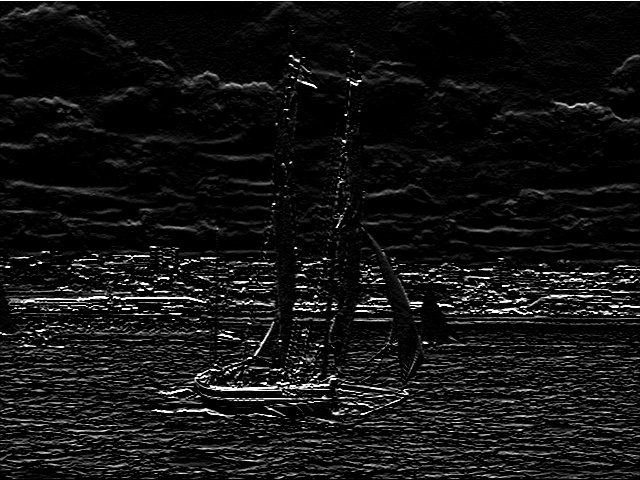
\includegraphics[width=0.8\textwidth]{IAcBBqAmEI_vertical-1.jpeg}
		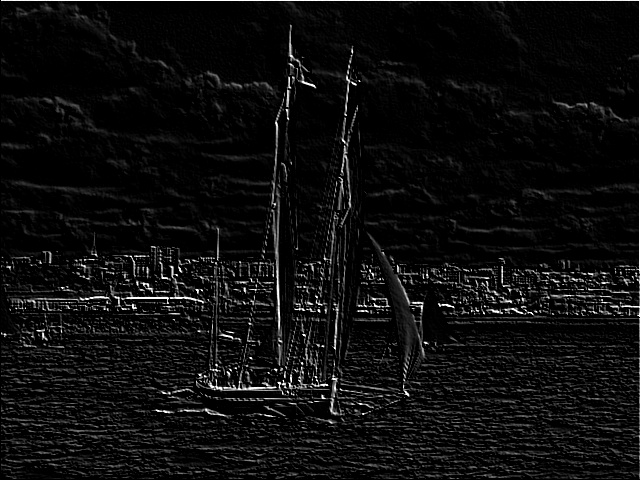
\includegraphics[width=0.8\textwidth]{IAcBBqAmEI_blended-1.jpeg}
		\captionsetup{width=.8\textwidth}
		\captionof{figure}{Horizontally, vertically filtered images and their blend, Filter-1}
	\end{minipage}
\end{minipage}

\begin{minipage}{\textwidth}
	\begin{minipage}{0.49\textwidth}
		\centering
		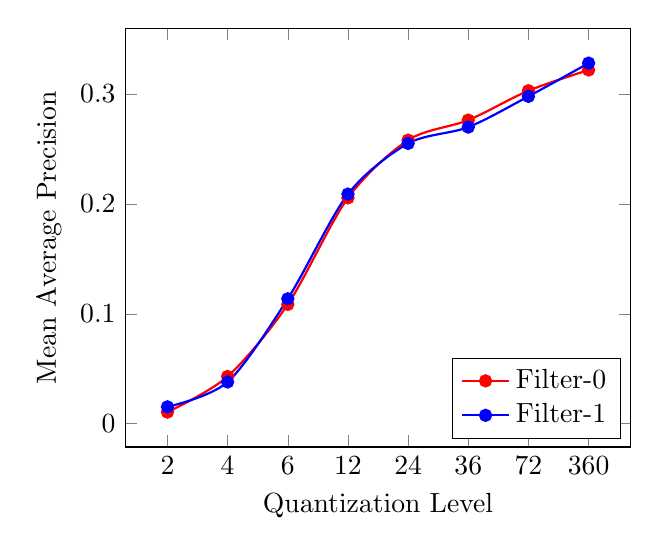
\begin{tikzpicture}
		    \begin{axis}
		        [
		        ,xlabel=Quantization Level
		        ,ylabel=Mean Average Precision
		        ,yticklabel style={/pgf/number format/fixed}
		        ,xtick=data
		        ,xticklabels={2, 4, 6, 12, 24, 36, 72, 360}
		        ,legend style={at={(0.98 ,0.02)},anchor=south east}
		        ]
		        \addplot [mark=*,smooth,red,thick] coordinates
		        {(0,0.01051) (1,0.04294) (2,0.10854) (3,0.20549) (4,0.25805) (5,0.27627) (6,0.30302) (7,0.32188)};
		        \addplot [mark=*,smooth,blue,thick] coordinates
		        {(0,0.01530) (1,0.03795) (2,0.11364) (3,0.20891) (4,0.25502) (5,0.26988) (6,0.29787) (7,0.32813)};
		        \legend{{Filter-0},{Filter-1}}[b];
		    \end{axis}
		\end{tikzpicture}
		\captionsetup{width=.9\textwidth}
		\captionof{figure}{Mean Average Precision with different quantization levels and filters for grid level 1 gradient histogram}
	 \end{minipage}
	 \hfill
	\begin{minipage}{0.49\textwidth}
		\centering
		\begin{tabular}{ | c | c | c | }
		  	\hline			
		  	\bf Bin & \bf Filter & \bf mAP \\
			\hline
		   	\multirow{2}{*}{2} & 0 & 0.01051 \\
		   	\cline{2-3}
		   	& 1 & 0.01530 \\
		  	\hline
		   	\multirow{2}{*}{4} & 0 & 0.04294 \\
		   	\cline{2-3}
		    & 1 & 0.03795 \\
		  	\hline
		   	\multirow{2}{*}{6} & 0 & 0.10854 \\
		   	\cline{2-3}
		    & 1 & 0.11364 \\
		  	\hline
		   	\multirow{2}{*}{12} & 0 & 0.20549 \\
		   	\cline{2-3}
		    & 1 & 0.20891 \\
		  	\hline
		   	\multirow{2}{*}{24} & 0 & 0.25805 \\
		   	\cline{2-3}
		    & 1 & 0.25502 \\
		  	\hline
		   	\multirow{2}{*}{36} & 0 & 0.27627 \\
		   	\cline{2-3}
		    & 1 & 0.26988 \\
		  	\hline
		   	\multirow{2}{*}{72} & 0 & 0.30302 \\
		   	\cline{2-3}
		   	& 1 & 0.29787 \\
		  	\hline
		  	\multirow{2}{*}{360} & 0 & 0.32188 \\
		   	\cline{2-3}
		   	& 1 & 0.32813 \\
		  	\hline
		\end{tabular}
		\captionsetup{width=.8\textwidth}
		\captionof{table}{Mean Average Precision with different quantization levels and filters for grid level 1 gradient histogram}
	\end{minipage}
\end{minipage}

%\newpage
%\textbf{Before starting the next section, please pick up the best configuration for three properties above and continue with them.}

\section{Grid Based Feature Extraction}
%Give your mAP for all of the configurations below.

\subsection{level 1}
\begin{minipage}{\textwidth}
	\begin{minipage}{0.49\textwidth}
		\centering
		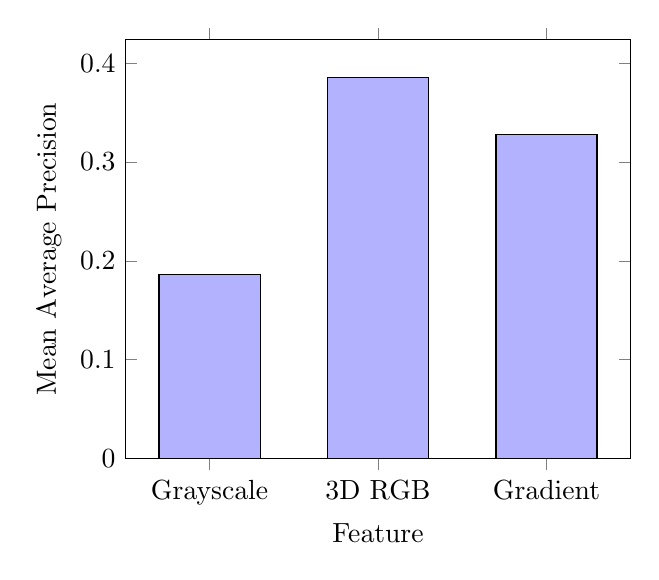
\begin{tikzpicture}
		    \begin{axis}
		        [
		        ,xlabel=Feature
		        ,ylabel=Mean Average Precision
		        ,ybar
		        ,bar width=0.6
		        ,xmin=-0.5,xmax=2.5
		        ,ymin=0
		        ,yticklabel style={/pgf/number format/fixed}
		        ,xtick=data,
		        ,xticklabels={Grayscale, 3D RGB, Gradient}
		        ]
		        \addplot [fill=blue!30] coordinates
		        {(0,0.18619) (1,0.38512) (2,0.32813)};
		    \end{axis}
		\end{tikzpicture}
		\captionsetup{width=.9\textwidth}
		\captionof{figure}{Best configurations of different features for grid level 1 in case of Mean Average Precision}
	 \end{minipage}
	 \hfill
	\begin{minipage}{0.49\textwidth}
		\centering
		\begin{tabular}{ | c | c | c | }
		  	\hline			
		  	\bf Bin & \bf Feature & \bf mAP \\
		  	\hline			
		  	16 & Grayscale & 0.18619 \\
		  	\hline			
		  	16 & 3D Color & 0.38512 \\
		  	\hline			
		  	360 & Gradient & 0.32813 \\
		  	\hline
		\end{tabular}
		\captionsetup{width=.8\textwidth}
		\captionof{table}{Best configurations of different features for grid level 1 in case of Mean Average Precision}
	\end{minipage}
\end{minipage}

\subsection{level 2}
\begin{minipage}{\textwidth}
	\begin{minipage}{0.49\textwidth}
		\centering
		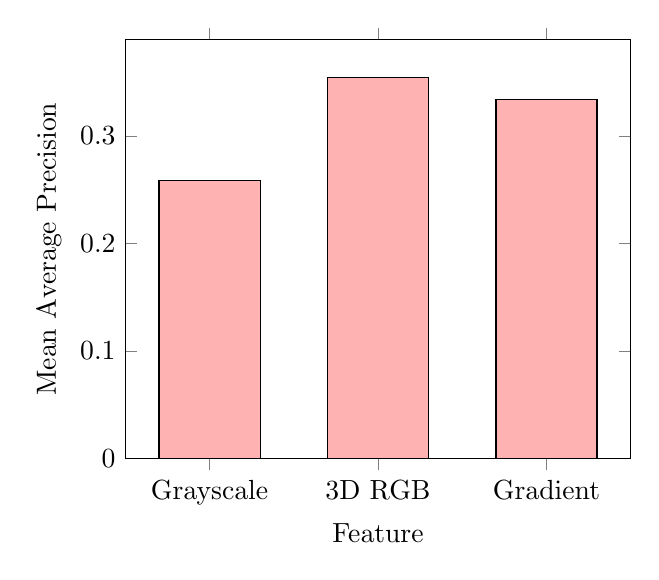
\begin{tikzpicture}
		    \begin{axis}
		        [
		        ,xlabel=Feature
		        ,ylabel=Mean Average Precision
		        ,ybar
		        ,bar width=0.6
		        ,xmin=-0.5,xmax=2.5
		        ,ymin=0
		        ,yticklabel style={/pgf/number format/fixed}
		        ,xtick=data,
		        ,xticklabels={Grayscale, 3D RGB, Gradient}
		        ]
		        \addplot [fill=red!30] coordinates
		        {(0,0.25874) (1,0.35405) (2,0.33385)};
		    \end{axis}
		\end{tikzpicture}
		\captionsetup{width=.9\textwidth}
		\captionof{figure}{Best configurations of different features for grid level 2 in case of Mean Average Precision}
	 \end{minipage}
	 \hfill
	\begin{minipage}{0.49\textwidth}
		\centering
		\begin{tabular}{ | c | c | c | }
		  	\hline			
		  	\bf Bin & \bf Feature & \bf mAP \\
		  	\hline			
		  	16 & Grayscale & 0.25874 \\
		  	\hline			
		  	16 & 3D Color & 0.35405 \\
		  	\hline			
		  	360 & Gradient & 0.33385 \\
		  	\hline
		\end{tabular}
		\captionsetup{width=.8\textwidth}
		\captionof{table}{Best configurations of different features for grid level 2 in case of Mean Average Precision}
	\end{minipage}
\end{minipage}

\subsection{level 3}
\begin{minipage}{\textwidth}
	\begin{minipage}{0.49\textwidth}
		\centering
		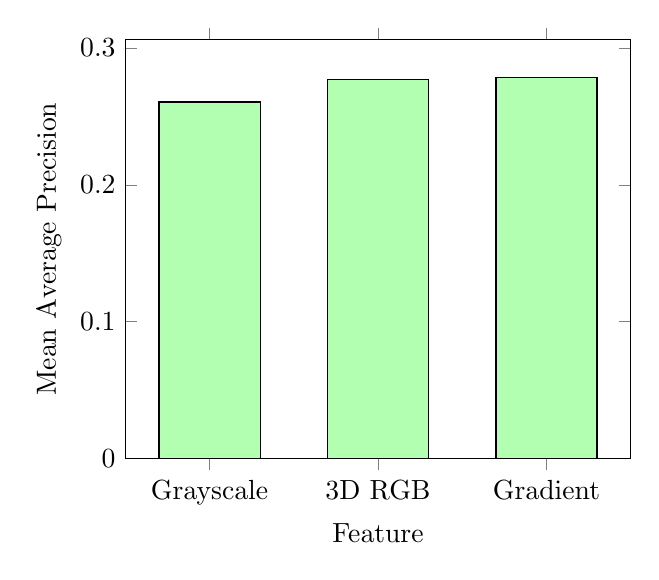
\begin{tikzpicture}
		    \begin{axis}
		        [
		        ,xlabel=Feature
		        ,ylabel=Mean Average Precision
		        ,ybar
		        ,bar width=0.6
		        ,xmin=-0.5,xmax=2.5
		        ,ymin=0
		        ,yticklabel style={/pgf/number format/fixed}
		        ,xtick=data,
		        ,xticklabels={Grayscale, 3D RGB, Gradient}
		        ]
		        \addplot [fill=green!30] coordinates
		        {(0,0.26052) (1,0.27730) (2,0.27822)};
		    \end{axis}
		\end{tikzpicture}
		\captionsetup{width=.9\textwidth}
		\captionof{figure}{Best configurations of different features for grid level 3 in case of Mean Average Precision}
	 \end{minipage}
	 \hfill
	\begin{minipage}{0.49\textwidth}
		\centering
		\begin{tabular}{ | c | c | c | }
		  	\hline			
		  	\bf Bin & \bf Feature & \bf mAP \\
		  	\hline			
		  	16 & Grayscale & 0.26052 \\
		  	\hline			
		  	16 & 3D Color & 0.27730 \\
		  	\hline			
		  	360 & Gradient & 0.27822 \\
		  	\hline
		\end{tabular}
		\captionsetup{width=.8\textwidth}
		\captionof{table}{Best configurations of different features for grid level 3 in case of Mean Average Precision}
	\end{minipage}
\end{minipage}

\subsection{questions}
\begin{itemize}
\item What do you think cause the difference between the results?
\item How did you combine the histograms in level 2 and 3? What would you think the difference between to simply sum them and to concatenate them?
\end{itemize}

\begin{minipage}{\textwidth}
	\begin{minipage}{0.49\textwidth}
		\centering
		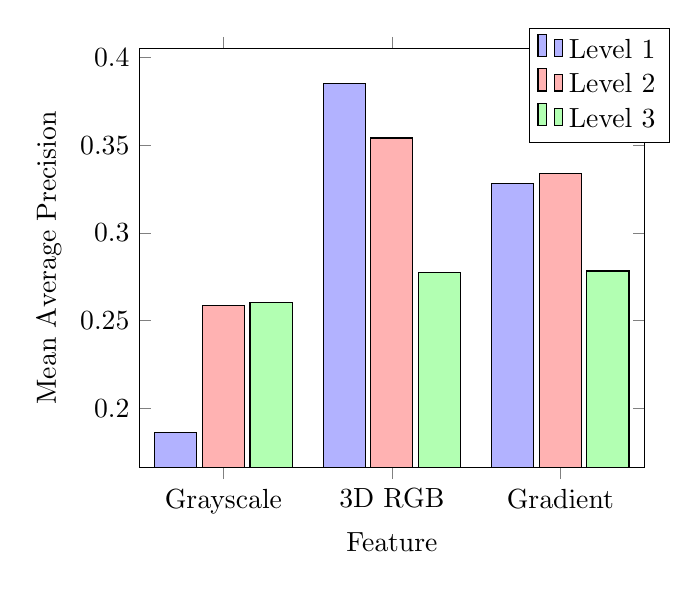
\begin{tikzpicture}
		    \begin{axis}
		        [
		        ,xlabel=Feature
		        ,ylabel=Mean Average Precision
		        ,yticklabel style={/pgf/number format/fixed}
		        ,ybar
		        ,bar width=0.25
		        ,xmin=-0.5, xmax=2.5
		        %,width=0.95\textwidth
		        ,xtick={0, 1, 2}
		        ,xticklabels={Grayscale, 3D RGB, Gradient}
		        ,legend style={at={(1.05 ,1.05)}}
		        ]
		        \addplot [fill=blue!30] coordinates
		        {(0,0.18619) (1,0.38512) (2,0.32813)};
		        \addplot [fill=red!30] coordinates
		        {(0,0.25874) (1,0.35405) (2,0.33385)};
		        \addplot [fill=green!30] coordinates
		        {(0,0.26052) (1,0.27730) (2,0.27822)};
		        %,\addplot [draw=none] coordinates
		        %,{(-0.5,0) (1,0) (2.5,0)};
		        \legend{{Level 1},{Level 2},{Level 3}}[b];
		    \end{axis}
		\end{tikzpicture}
		\captionsetup{width=.9\textwidth}
		\captionof{figure}{Mean Average Precision comparison among different features in different grid levels with level 1 best configurations}
	 \end{minipage}
	 \hfill
	\begin{minipage}{0.49\textwidth}
		\centering
		\begin{tabular}{ | c | c | c | c | }
		  	\hline			
		  	\bf Level & \bf Bin & \bf Feature & \bf mAP \\
			\hline
			\multirow{3}{*}{1} & 16 & Grayscale & 0.18619 \\
		   	\cline{2-4}
		   	& 16 & 3D Color & 0.38512 \\
		   	\cline{2-4}
		   	& 360 & Gradient & 0.32813 \\
			\hline
		   	\multirow{3}{*}{2} & 16 & Grayscale & 0.25874 \\
		   	\cline{2-4}
		   	& 16 & 3D Color & 0.35405 \\
		   	\cline{2-4}
		   	& 360 & Gradient & 0.33385 \\
			\hline
		   	\multirow{3}{*}{3} & 16 & Grayscale & 0.26052 \\
		   	\cline{2-4}
		   	& 16 & 3D Color & 0.27730 \\
		   	\cline{2-4}
		   	& 360 & Gradient & 0.27822 \\
		   	\hline
		\end{tabular}
		\captionsetup{width=.8\textwidth}
		\captionof{table}{Mean Average Precision comparison table of different features with feature's best level 1 configuration and with different grid levels}
	\end{minipage}
\end{minipage}

\section{Your Best Configuration}
\begin{itemize}
\item You may try different combinations including changing parameters above and even combining different methods. Simply give your best mAP for the validation set:


\item Explain your setup for this best mAP. How can we reproduce your result using your code?

\item Give some visual ranking results:

\item Explain mean average precision in your own words:
\end{itemize}

\section{Additional Comments and References}

(if there any)





\end{document}


\grid
\grid
